¿Cuál es el \'area del paralelogramo de la figura \ref{fig:area_compuesta_01}?

\begin{figure}[H]
    \begin{center}
        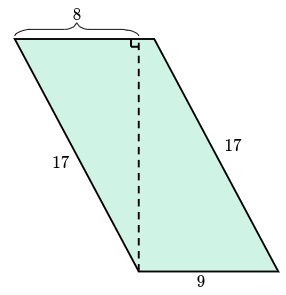
\includegraphics[width=0.25\linewidth]{../images/area_compuesta_01.png}
    \end{center}
    \caption{}
    \label{fig:area_compuesta_01}
\end{figure}
\begin{solutionbox}{13cm}

    \begin{minipage}{0.6\textwidth}
        Para determinar el área del paralelogramo debemos saber la longitud del cateto del triángulo rectángulo. Llamemos $x$ a la longitud (ver Figura \ref{fig:area_compuesta_01a}).
        Cuando tenemos un triángulo rectángulo, podemos usar el teorema de Pitágoras para obtener la longitud del cateto.
        La ecuación para el teorema de Pitágoras es:
        \[c^2=a^2+b^2\]
        En este caso, $a=8$, $b=x$ y $c=17$, Entonces,
        \begin{align*}
            8^2+x^2 & =17^2   \\
            64+x^2  & =289    \\
            x^2     & =289-64 \\
            x^2     & =225    \\
            x       & =15
        \end{align*}
        La base del paralelogramo es 9 y la altura 15. El área del paralelogramo es:

        \begin{align*}
            A & =bx              \\
            A & =9\cdot 15       \\
            A & =135 \text{ u}^2
        \end{align*}
    \end{minipage}\hfill
    \begin{minipage}{0.35\textwidth}
        \begin{figure}[H]
            \centering
            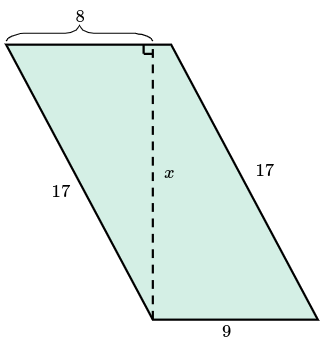
\includegraphics[width=0.9\linewidth]{../images/area_compuesta_01a.png}
            \caption{}
            \label{fig:area_compuesta_01a}
        \end{figure}
    \end{minipage}

\end{solutionbox}